%% ----------------------------------------------------------------------------
% BIWI SA/MA thesis template
%
% Created 09/29/2006 by Andreas Ess
% Extended 13/02/2009 by Jan Lesniak - jlesniak@vision.ee.ethz.ch
%% ----------------------------------------------------------------------------
\documentclass[a4paper,12pt,twoside]{report} %openright {book}

\usepackage[dvipsnames]{xcolor}
\usepackage[backend=biber,
            autocite=superscript,
            sorting=none,
            url=false
            ]{biblatex}
\usepackage{csquotes}
\usepackage[english]{babel}
\usepackage[parfill]{parskip}
\usepackage[pdfauthor={Koen Wolters},
            pdftitle={Semester Project},
            plainpages=false,
            pdfpagelabels,
            colorlinks=true,
            linkcolor=blue,
            bookmarks=true,
            filecolor=blue,
            urlcolor=blue,
            citecolor=blue
           ]{hyperref}

\usepackage[headheight=110pt,left=1.5in,right=1.5in,top=1.5in,bottom=1.5in]{geometry}
\usepackage{graphicx}		% For including images
\usepackage{fancyhdr}		% Produce the nice header

\usepackage{paralist}		% List environment
\usepackage{color}		% For colored text
\usepackage{times}
\usepackage{amsfonts}		% Additional math fonts
\usepackage{amsmath}		% Math symbols
\usepackage{latexsym}
% \usepackage{listings}		% If listings are needed
\usepackage{mydefs}		% Some of our own definitions
% \usepackage{wrapfig}		% To wrap images
% \usepackage{algorithmic}	% Nice algorithm environment
% \usepackage{algorithm}

% TODO
%\newcommand{\needref}{~[REF?]}
%\newcommand{\needfig}{~[FIG?]}
%\newcommand{\needref}{}
%\newcommand{\needfig}{}


% Change the appearance of the header. Here \MakeUppercase is hard-coded, so renewing this command allows to elegantly change the header appearance.
\renewcommand{\MakeUppercase}{\scshape}

\fancypagestyle{plain}{
  \renewcommand{\headrulewidth}{0.0pt}
  \fancyfoot{}
  \fancyhead{}
}

\fancyfoot{}
\fancyhead[RO,LE]{\thepage}
\fancyhead[LO]{\leftmark}
\fancyhead[RE]{\rightmark}

\pagestyle{fancy}

\setlength{\fboxsep}{0pt}%
%\setlength{\headheight}{55pt}
%\addtolength\topmargin{-10pt}
%\addtolength\footskip{20pt}

\addbibresource{references.bib}

% The first pages shall be empty, even no page numbering 
\begin{document}
\hypersetup{pageanchor=false}
% Title page, modify accordingly 
%% ----------------------------------------------------------------------------
% BIWI SA/MA thesis template
%
% Created 09/29/2006 by Andreas Ess
% Extended 13/02/2009 by Jan Lesniak - jlesniak@vision.ee.ethz.ch
%% ----------------------------------------------------------------------------

\begin{titlepage}

\thispagestyle{empty}

\fancypagestyle{empty}{
\lhead{\vspace{2cm}
\includegraphics[height=1.7cm]{images/ethlogo_black}}
\renewcommand{\headrulewidth}{0.0pt}
\rhead{
\includegraphics[height=1.7cm]{images/cvl_logo}\hspace{0.2cm}
\includegraphics[height=1.7cm]{images/cvl_acronym}}
\fancyfoot{}
}



\vspace*{2cm}
\begin{center}
\Huge{\textbf{Self-supervised learning with an ordering task on an autonomous driving dataset}\\}
\vspace*{3mm}
\Large{\textbf{Learning from camera and lidar data}\\[1cm]}

\large{Semester Project\\[0.8cm]}
\LARGE{Koen Wolters\\}
\normalsize{Department of Electrical Engineering \& Information Technology}
\end{center}

\begin{center}
 


% \begin{center}
% \begin{tabular}{ll}
% \multirow{2}{*}{
\includegraphics[height=1cm]{images/biwi_logo}} & Computer Vision Laboratory\\ 
% & ETH Zurich
% \end{tabular}
%  \end{center}

\end{center}


\vfill
\begin{center}
\begin{tabular}{ll}
%\Large{\textbf Advisor:} &
\Large{\textbf Supervisors:} &  \Large{Dr.~Dengxin~Dai}\\ 
                             &  \Large{Prof.~Dr.~Luc van Gool}\\
 			    & \small{Computer Vision Laboratory}\\
			    & \small{Department of Information Technology and Electrical Engineering}\\
\end{tabular}
\end{center}

\begin{center}
\today\\
\end{center}


\end{titlepage}

%\clearpage

%% ----------------------------------------------------------------------------
% BIWI SA/MA thesis template
%
% Created 09/29/2006 by Andreas Ess
% Extended 13/02/2009 by Jan Lesniak - jlesniak@vision.ee.ethz.ch
%% ----------------------------------------------------------------------------

\newpage
\vspace{3cm}

\chapter*{Abstract}
Convolutional neural networks have achieved strong results over the last decade. However with networks typically having milions of parameters, large labeled datasets are needed to learn powerful generalizable models and constructing those supervision signals is hampered by the expense of human annotation required. Self-supervised learning is a novel paradigm exploiting the intrinsic structure of data to create labels automatically, aiming to learn generic features. Videos from car dataset for autonomous driving contain much intrinsic data from camera and lidar sensors and pose an interesting possibility for a self-supervised ordering task. 

This work aims to do an initial study of the learning performance of this ordering task on the Kitti dataset, without using its annotation. Frames are shuffled and both an easier task, where the network has to estimate if the data is sorted or not, as well as a harder task to estimate the permutation, are explored. As input features camera and lidar data are sampled with images in color and grayscale, and lidar with projected 2D depth, height and reflectances maps.

It has been found that neural networks are well capable of sorting the video frames, with top-1 accuracies close to 60\% on the harder permutation estimation ordering task. In particular it is shown that the interpolated lidar depth serves as a strong feature. More remarkably, combining lidar and camera data does not lead to a significant improvement in accuracy as has been hypothesized, although this might have been caused by a too small set of training data.

While the network learns basic generic filters, needed for achieving the high accuracy on the task itself, the network does only seem to learn limited high-level features. The quality of the learned features do therefore not seem to be strong enough to transfer the learning to other domains yet, but self-supervision has been shown to be a promising direction of future research to enhance the learning of classification networks and driving models for autonomous cars.

%In this work we study the application of recent self-supervised learning techniques on datasets for autonomous driving. The focus of this work is the usage of temporal coherence to learn to predict order and coherence between lidar and camera images.

%[...]
% \noindent The abstract gives a concise overview of the work you have done. The reader shall be able to decide whether the work which has been done is interesting for him by reading the abstract. Provide a brief account on the following questions:
% 
% \begin{itemize}
%  \item What is the problem you worked on? (Introduction)
%  \item How did you tackle the problem? (Materials and Methods)
%  \item What were your results and findings? (Results)
%  \item Why are your findings significant? (Conclusion)
% \end{itemize}
% 
% \noindent The abstract should approximately cover half of a page, and does generally not contain citations.




% Input here any acknowledgements
%% ----------------------------------------------------------------------------
% BIWI SA/MA thesis template
%
% Created 09/29/2006 by Andreas Ess
% Extended 13/02/2009 by Jan Lesniak - jlesniak@vision.ee.ethz.ch
%% ----------------------------------------------------------------------------


\newpage

\chapter*{Acknowledgements}
I would like to thank Prof. Dr. Luc van Gool for offering me the opportunity to do a semester project in the CVL group. 

My special thanks goes to my direct supervisor Dr. Dengxin Dai for his advice and assistance during the course of this semester project. Moreover, I wish to acknowledge the help provided by Vaishakh Patil with preparing the input feature maps.

Finally I would like to offer my great appreciation to my parents for their never-ending enthusiasm and support throughout my study. 



\clearpage
\newpage

% % Chapter-pages etc. use the ``plain'' pagestyle - since we don't want to have a heading at all at chapter-pages, redefine plain accordingly. Don't forget the page number. 
% \fancypagestyle{plain}{
%   \renewcommand{\headrulewidth}{0.0pt}
%   \fancyfoot{}
%   \fancyfoot[RO, LE]{\thepage} % E
%   \fancyhead{}
% }

\hypersetup{pageanchor=false}
\pagenumbering{Roman}

% Insert table of contents
\tableofcontents

% Insert list of figures
%\listoffigures
\clearpage

% Insert list of tables
%\listoftables
\clearpage

\newpage

\pagenumbering{arabic}

%% ----------------------------------------------------------------------------
% Actual text comes here - defer it to other files and use \input{bla.tex}, ..
%% ----------------------------------------------------------------------------
%% ----------------------------------------------------------------------------
% BIWI SA/MA thesis template
%
% Created 09/29/2006 by Andreas Ess
% Extended 13/02/2009 by Jan Lesniak - jlesniak@vision.ee.ethz.ch
%% ----------------------------------------------------------------------------

% Give an introduction to the topic you have worked on:
% 
% \begin{itemize}
%  \item \textit{What is the rationale for your work?} Give a sufficient description of the problem, e.g. with a general description of the problem setting, narrowing down to the particular problem you have been working on in your thesis. Allow the reader to understand the problem setting. 
%  \item \textit{What is the scope of your work?} Given the above background, state briefly the focus of the work, what and how you did.
%  \item \textit{How is your thesis organized?} It helps the reader to pick the interesting points by providing a small text or graph which outlines the organization of the thesis. The structure given in this document shows how the general structuring shall look like. However, you may fuse chapters or change their names according to the requirements of your thesis.
% \end{itemize}

\chapter{Introduction}
With the increase of computational power the field of computer vision has made huge leaps forward in recent years. The integration of machine learning techniques and especially the introduction of deep Convolutional Neural Networks (CNN) allowed for unparalleled performance on classification and detection tasks~\cite{krizhevsky2012}. Convolutional neural network do not only automate feature selection and classification, but also feature design which has been a complicated topic in computer vision research over the years\needref. Neural networks provide a large learning capacity and the capability to learn every type of function. However, with several milions of parameters, those networks need large labeled datasets to prevent overfitting and to learn powerful generalizable models.

Nowadays datasets like Imagenet provide millions of labeled images in over thousands of categories~\cite{deng2009}, overcoming earlier shortcomings of smaller datasets. Efforts to scale these methods to billions of images are however hampered by the expense of human annotation required~\cite{doersch2015}, limiting possibilities for improvements in the future. The costly and time-consuming process of manual annotation harms the scalability to new problem domains in particular, especially for tasks involving more complex data (like videos and 3D imaging \needref) and tasks requiring expertise~\cite{lee2017,fernando2017}. In this context it would be legitimate to ask: do we really need strong-supervision from so many images to train those CNNs~\cite{wang2015}?

Unfortunately, despites decades of sustained effort, unsupervised learning have not yet reached the level to allow it to extract useful information from large collection of full-size images~\cite{doersch2015}. Humans however excel in inferring 3D structure and developing a strong belief of structure also in short timescales, while receiving only limited semantic supervision. One hypothesis of the reason humans perform so well in this task is that we develop a rich structural understanding of the world through past visual experience and creating consistent modeling of our observations~\cite{zhou2017}. In this way the context has shown to be an important factor in learning, which leads to the concept of self-supervised learning.

Self-supervised learning is the use of all the 'free' data on the web and exploits its intrinsic structure for training neural networks. Self-supervised learning techniques can exploit reward signals from both both spatial coherence, for example by learning the correct location of patches~\cite{doersch2015, noroozi2016}, as well as temporal coherence, for example by learning to order frames in videos~\cite{misra2016, lee2017}. Although these tasks are rather specialized, these self-taught features can often generalize well to a certain extent. By using transfer learning the performance on supervised tasks can be improved, as the networks learn similar basic visual patterns required for classification~\cite{raina2007}. In the framework of CNNs this optimization procedure is usually referred to a 'fine-tuning', giving similar classification performance with much less supervision \needref.

Autonomous driving has recently seen a huge interest both from a commercial perspective as well as in robotics research. This topic is closely related to the field of computer vision, with detection of objects like cars, pedestrians and signs being a major part allowing to drive autonomously. The application of convolutional neural networks has achieved huge success in improving object detection \needref, but suffers again from the requirement of huge annotated datasets for sufficient performance \needref. Various datasets like the Kitti~\cite{geiger2012} and the Oxford Robotcar~\cite{maddern2017} dataset contain driving videos with cameras from various perspectives, combined with high-quality lidar measurements, precise GPS tagging and accurate timing. These datasets therefore have extensive intrinsic structure and should thus be an excellent source for self-supervised learning. 

\section{Focus of this Work}
This work tries to take advantage of the free data in driving datasets. The expensive labeling in those datasets is not used, but instead self-supervising techniques are explored to learn features. The core of this report is the use of an order-prediction task to learn the temporal coherence between lidar and camera images and experiments to validate the generalization of the features learned in such a network.

\section{Thesis Organization}
This thesis is organized in several sections. Section \ref{ch:related_work} contains a literature research to related work in self-supervised learning and the application of lidar and gps signals for learning. In Section \ref{ch:materialsandmethods} the general neural network and researched variations are put forward. The performance of the neural network and the application of the learned model to other tasks are presented in Section \ref{ch:experimentsandresults}, followed by a detailed discussion in Section \ref{ch:discussion}.

%% ----------------------------------------------------------------------------
% BIWI SA/MA thesis template
%
% Created 09/29/2006 by Andreas Ess
% Extended 13/02/2009 by Jan Lesniak - jlesniak@vision.ee.ethz.ch
%% ----------------------------------------------------------------------------
\newpage
\chapter{Related Work}
\label{ch:related_work}
Unsupervised learning has been studied extensively over the past decades. Before the arrival of CNNs handcrafted features like SIFT, HOG and SURF have been used for classification and detection~\cite{lee2017}\needref. With deep learning visual representations can be extracted directly from data, but a network often requires millions of labeled images for the supervised learning. In a typical way of working CNNs are trained on ImageNet~\cite{deng2009} and then afterwards fine-tuned for a more specific application with limited sources of supervision. 

There are various approaches to circumvent the problem with building supervisised datasets, learning in an unsupervised way instead. In reconstruction-based learning a network tries to learn representation that can reproduce itself, in self-supervised learning context is exploited as supervisory signal.

\section{Reconstruction-based learning}
In a more general sense, we can think of a good image representation as the latent variables of a generative model, but directly inferring this structure is generally intracable~\cite{doersch2015}. One well-researched way to approximate the model is using restricted Boltzmann machines, an generative stochastic artificial neural network trained in various forward and backward passes. In a restricted Boltmann machine there are hidden units that are activated by a stochastic weighted model over the input nodes, and those activations are passed backward in an attempt to reconstruct the input, learning the weights by minimizing reconstruction error~\cite{smolensky1986}. 

Another interesting approach, which works by similar means, is auto-encoding, where the input image also functions as the output of the network. To build useful features in the hidden layers and thus to prevent learning the identity function, images are corrupted with the task of the network being to denoise and reconstruct the original image. Often a sparsity penalty is added to allow the technique to be applied in deep networks. It was shown that this approach makes it possible to make robust human body detectors without lableling, but using full-sized images such a network required up to a million CPU hours to learn some valuable representations~\cite{le2013}.  

\section{Self-supervised learning}
Self-supervised learning is another novel unsupervied learning paradigm that exploits different labelings that are freely available besides or within visual data. Those labelings are usually of limited direct interest to estimate during test time. Instead those sources are often processed as a pretext task with the goal of learning general features that can later be remodelled for vision tasks such as object detection and semantic segmentation\needref. To achieve this, the networks used by those proposed tasks have a common convolutional backbone pipeline extracting features for object detection. Common choices for this multi-layer detection architecture include AlexNet~\cite{krizhevsky2012} (and the closely related CaffeNet~\cite{jia2014}), VGC~\cite{simonyan2014}, GoogleNet~\cite{szegedy2015} and ResNet~\cite{he2016}. For segmantic segmentation the pre-trained architectures can be integrated into a complete convolutational classification framework like the state-of-the-art Mask R-CNN~\cite{he2017} with the weights initialized to those from the self-supervised tasks. Finally smaller supervised datasets with full segmentations can then be used to train the network for classification and segmentation.

Recent work has investigated different sources of intrinsic information within image and video data that can be exploited for self-supervision. Most works have focused on the following main origins of context: 
\begin{itemize}
\item Spatial structure
\item Spatioemporal coherence 
\item Auxilliary data mostly in the form of egomotion.
\end{itemize}

\begin{figure}[t]
\centering
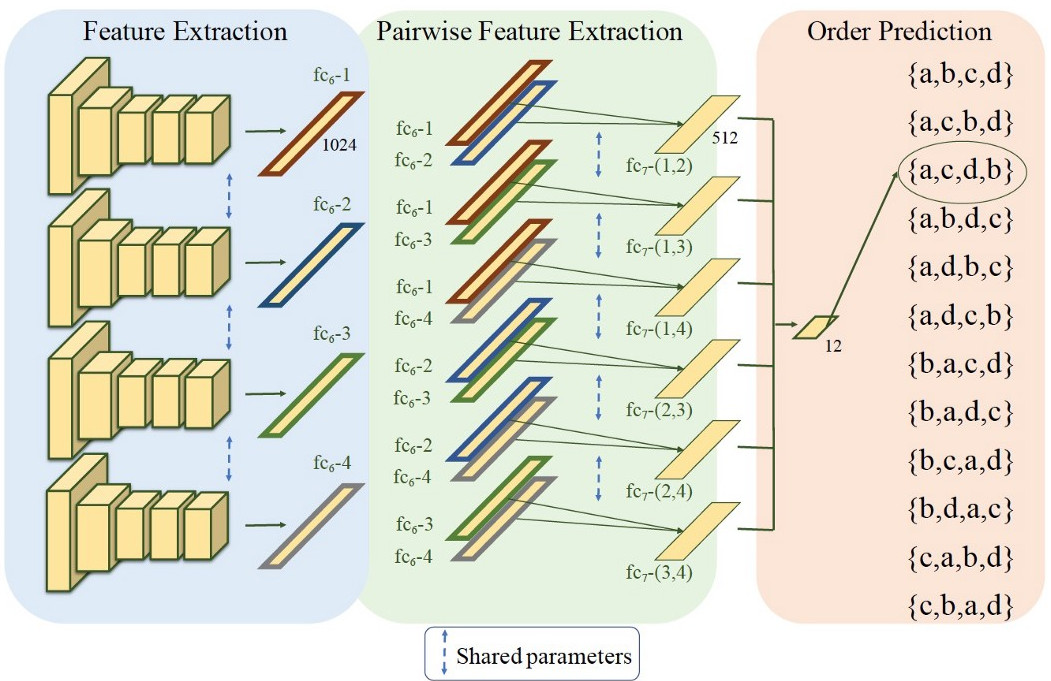
\includegraphics[width=\textwidth]{images/sorting_sequences.jpg}
\caption{Network proposed by Lee et al.\cite{lee2017} to sort a sequence of images. The four shuffled images enter on the right side and the output is a single integer representing a particular permutation. Image is modified from \cite{lee2017}.}
\label{fig:sorting_sequence}
\end{figure}

Doersch et al.~\cite{doersch2015} formulate a self-supervised task to learn spatial context in images. The image is first split in an 3x3 grid, and the patch in the middle of the image is taken together with any of the other 8 tiles. Then the network is trained to learn to predict the correct location of the second tile relative to the first. This work was later extended to observe all the tiles at the same time by shuffling the patches and learning to solve the created jigsaw puzzle~\cite{noroozi2016}, an example shown earlier in Figure \ref{fig:jigsaw}. Another related technique was put forward by Wang \& Cupta~\cite{wang2015} that tries to exploit different views of the same object and use known similarity as a training loss. It does this by mining two images of the same object, found using unsupervised KLT-tracking with SURF features in video data, and another totally unrelated random image. The setup uses a Siamese network for the three images with the final loss penalizing differences in the visual representation of the same object and on the opposite side similarities in comparison with the random image.

This last approach makes use of temporal coherence, but is ultimately an spatial learning method requiring significant pre-processing to create the similarity task. Misra et al.~\cite{misra2016} opt for an easier way to learn directly from the temporal coherence. They mine sequences of three frames from videos and shuffle these in a random order, using the fact if the permutation is sorted or not as supervision source. This approach was expanded later to sequences of longer length with the task of the neural network to learn the full permutation by Lee et al.~\cite{lee2017}. Their network uses a Caffenet\cite{jia2014} CNN in a Siamese structure for independent feature extraction in the backbone network ending in a single fully connected layer of 1024 neurons, followed by pair-wise feature extraction between all the fully connected layers that combines into a set of 512 neurons layer, and ending in a final fully-connected output layer for the actual order prediction. This network is shown in more detail graphically in Figure \ref{fig:sorting_sequence} as will be an important base for this work. In another variation of temporal coherence, a network is fed $N$ correctly ordered tuples and one other in the wrong order. The network can then try to learn to identify the wrongly ordered tuple in all $N+1$ tuple inputs~\cite{fernando2017}. Both approaches makes the learning formulation more complicated, allowing learning richer representations\needref. 

A final interesting form of supervision is ego-motion, which include the information about movement as recorded by other sensors. Living species also leverage self-generated movement in concert with visual feedback for proper perceptual development. Inspired by this concept, neural networks should also be able to benefit from information from motoral activity. Agrawal et al.~\cite{agrawal2015} directly use information about camera transformations, their agent optimizes it visual representations by minimizing the error between the egomotion obtained from the motor system and egomotion predicted using the network only. The two image frames go through a Siamese base architecture followed by fully-connected layers to estimate the transformation. In a similar work Jayaraman \& Grauman~\cite{jayaraman2015} learn a equivariant feature space using ego-motion by mapping the feature space between two frames and calculating the loss based on the difference between the features.

\section{Using 3D lidar data in CNNs}
Earlier work on self-supervision has focused on images, videos and auxilliary signals in the form of egomotion. This work aims to integrate lidar data to optimize the performance of the network. While lidar data has not been actively applied in the context of self-supervision and historically general focus in object detection has been on RGB images, various earlier works have already investigated the usage of lidar data. Because lidar data is intrinsically 3D it cannot be handled directly by an 2D neural network. The logical step of adding an extra channel to make the convolutions 3D, will likely work from a theoretical perspective, but implemented in a naive way will be computationally very expensive, and requires huge amounts of memory. A key finding to optimize the performance is the observation that lidar data is sparse and most of the space is unoccupied\cite{wang2015vote}, showing possibilities to simplify convolutions significantly by exploiting a duality between sliding window detection with linear classifiers and a voting scheme only from the occupied cells. This approach was later optimized with rectified linear units and a $\Lambda_1$ penalty to improve layer sparsity over the entire CNN stack\cite{engelcke2017}. A similar proposal was put forward by Zhou et al~\cite{zhou2017voxelnet} to combining point-wise features with a locally aggregrated feature in the form of a 3D voxel. 

In prior works~\cite{engelcke2017,zhou2017voxelnet,wang2015} using 3D convolutions the focus is on estimating 3D bounding boxes and semantic segmentation, however in our task the lidar data is only used as supplementary signal to boost the learning. As the addition of full 3D data is expected to be relatively marginal, and these approaches remain computationally expensive\needref\cite{chen2017} an alternative way is to project and discretize the 3D data to 2D front view \cite{li2016}. This approach can also be extended to a multi-view approach, generating both a bird-eye view and a front-view as been put forward by Chen et al.~\cite{chen2017}. The usage of 2D projection schemes for lidars is simpler to combine with image data, as it allows fusing the data from the different networks at different layers of the backbone network. Different fusion schemes have been explored with direct fusion by adding channels to the RGB channel, fusing at early layers and fusing at later layers~\cite{schlosser2016} spitting up the network views in different ways. Deep fusion has been proposed as well by continously combining and splitting the data at different layers~\cite{chen2017}.  

Before fusing the different layers, a initial question arises how to handle the projected 2D information generated from the lidars. The data projected at different layers will be sparse, leading to many empty cells when discretization is on the same order of magnitude as the image data. For the distances there is no natural way to handle missing data, as the logical initialization value of zero would indicate an object directly in front of the camera, which is often far from correct. Dolson et al.~\cite{dolson2010} propose a method to generate an interpolated depth map using Gaussian interpolation framework in high-dimensional spaces, regularizing the generation of a solution from sparse range data using camera frames to exploit the property that depth discontunities tend to align in intensity boundaries. An alternative upsampling method by Premebida et al.\cite{premebida2014} generates an dense depth map solely from the sparse range data by simply estimating the depth at a certain pixel as a weighted sum of points from within a certain neighbourhood, based on their distance to the pixel and their intensity values (giving higher priority to close detections). This approach gives less sharper boundaries, but is also more rigid to corruption of the depth signal.  

Naturally the lidar data contains information about distances - next to the reflectance values - however it is not directly clear if it best to learn directly from the depth map. Are there transformations of the input that the CNN learns more effectively from? Work by Gupta et al.~\cite{gupta2014} on RGB-D images suggests the use of a so-called HHA encoding, which transforms the depth map into a horizontal disparity map, the height above ground and the angle the pixel's local surface makes with the inferred gravity direction. More details about the construction of these features are given in an earlier work\cite{gupta2013}. Schossler et al.\cite{schlosser2016} use this HHA encoding on the depth maps from lidar data generated using the earlier-mentioned weighted upsampling method\cite{premebida2014} for the purpose of accurate detection of pedestrians.

%% ----------------------------------------------------------------------------
% BIWI SA/MA thesis template
%
% Created 09/29/2006 by Andreas Ess
% Extended 13/02/2009 by Jan Lesniak - jlesniak@vision.ee.ethz.ch
%% ----------------------------------------------------------------------------
\newpage
\chapter{Approach and Implementation}
\label{ch:approach_implementation}
The main goal of this paper is to investigate a self-supervised technique on autonomous driving videos using CNN's, with an self-supervised ordering task exploiting spatiotemporal signals. In the rest of this thesis we use a similar basic approach as in previous works on using temporal coherence~\cite{misra2016,lee2017}, but then applied to videos captured by cars. As a novel line of research the usage of lidar data is explored with the aim of learning richer representations. Different versions of the task are investigated as explained in more detail in the Chapter \ref{ch:experimentsandresults}, but the basic idea of the task is as follows:
\begin{enumerate}    
\item A sequence of images is selected with sufficient motion
\item The sequence is split into separate samples with different feature maps and fed individually through one or more siamese backbone networks merged at different depths with the goal of learning generic image features.
\item The output features of all images in the sequence are subsequently used as input to an ordering network.
\item The ordering network predicts either if the ordering is correct (easy)\cite{misra2016} or the actual permutation (harder)\cite{lee2017}.
\end{enumerate}
A general implementation of this approach for the permutation order network has been provided in Figure \ref{fig:sorting_sequence}.

\section{Generating train and test data}
\begin{figure}[t]
\centering
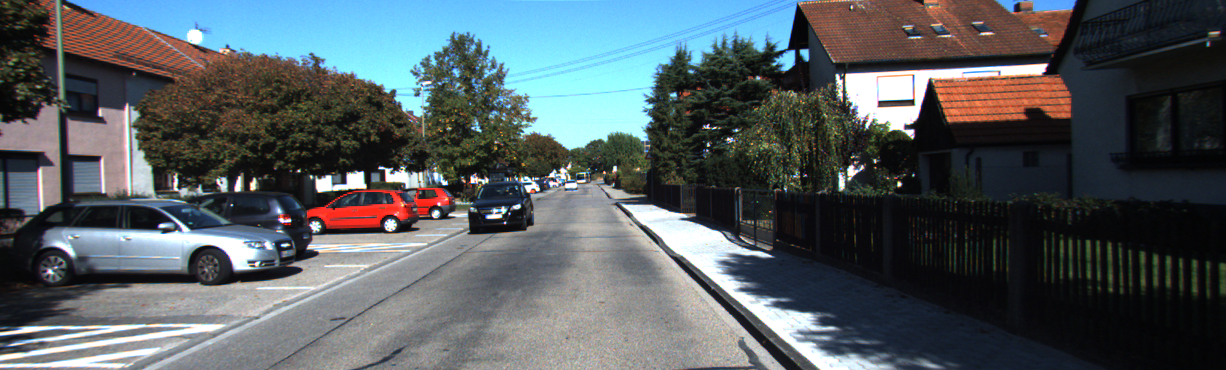
\includegraphics[width=\textwidth]{images/img_first.png}
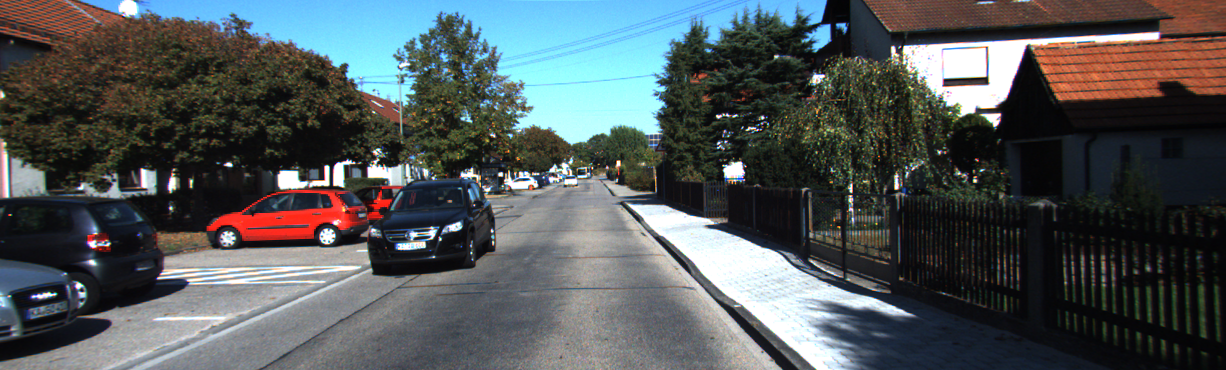
\includegraphics[width=\textwidth]{images/img_second.png}
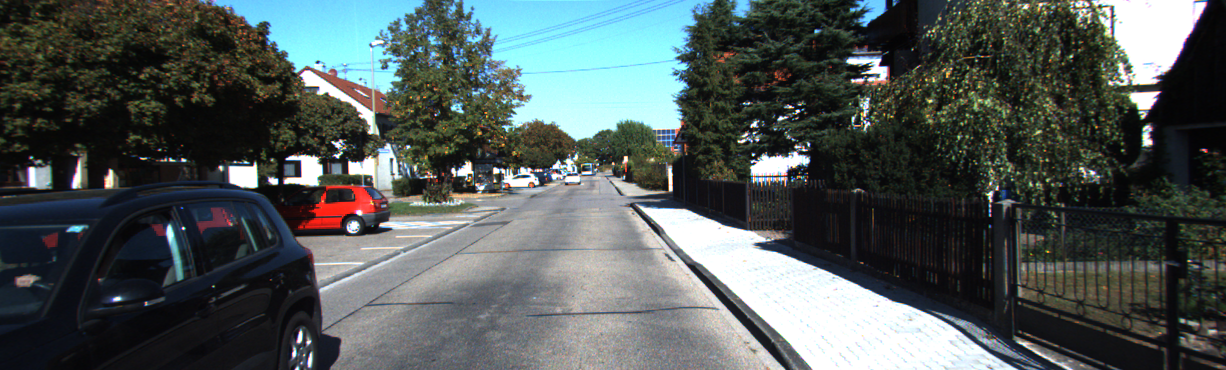
\includegraphics[width=\textwidth]{images/img_third.png}
\caption{Example of a sequence with three frames from the Kitti dataset~\cite{geiger2012}}
\label{fig:frames}
\end{figure}

As the task is unsupervised there is no need for labeled data, only a large number of video samples with precise lidar measurement. For this task one suitable choice is the Kitti\cite{geiger2012} visual odometry dataset, which is used in all experiments as it contains a large number of samples. This dataset contains a total of 22 sequences covering a total length of 39.2 km of outdoor streets divided in over 41k frames sampled at 10 Hz. It contains high-quality images from two grayscale and two color PointGrey Flea2 video cameras with 1392×512 pixel resolutions and corresponding lidar range scans from a Velodyne HDL-64E 3D laser scanner.

\begin{figure}
\centering
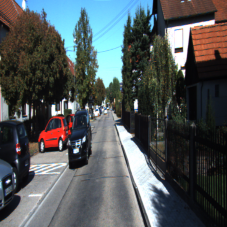
\includegraphics[width=0.49\textwidth]{images/color.png}
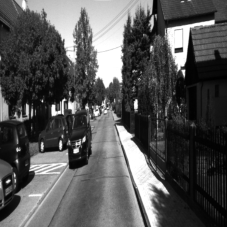
\includegraphics[width=0.49\textwidth]{images/gray.png}
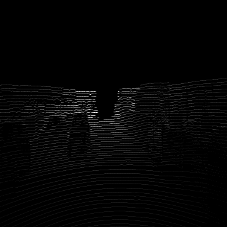
\includegraphics[width=0.49\textwidth]{images/lidar_depth.png}
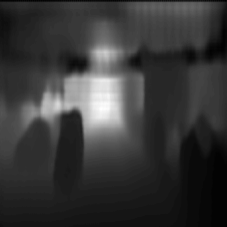
\includegraphics[width=0.49\textwidth]{images/lidar_depth_int.png}
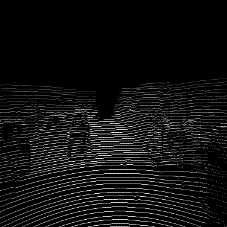
\includegraphics[width=0.49\textwidth]{images/lidar_height.png}
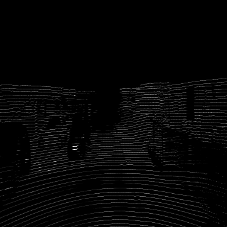
\includegraphics[width=0.49\textwidth]{images/lidar_refl.png}
\caption{Different representations of available data for the second frame displayed in Figure \ref{fig:frames} downscaled to the 227x227 version fed to the network before jittering is applied, with from top-left to bottom-right: color, grayscale, lidar depth, interpolated lidar depth, lidar height and lidar reflectance}
\label{fig:features}
\end{figure}

The dataset was split into 15 sequences for generating the training data and 7 independent sequences for testing. For generating the image data the RGB camera 02 was selected, the data from the other camera's was not used. Because the input images are of large dimensions for common backbone networks the images were first downscaled with anti-aliasing to a size of 227x227 as used in Caffenet~\cite{jia2014}. This resizing does not preserve scaling, but this is not a primary issue as all images are downsized in the same way and the structure of the objects remain clear in those smaller images. Finally for all experiments with single channel camera images, channel splitting is employed by randomly selecting one of the three RGB channels, it has been shown that this makes the data more rigid against learning low-level features then direct conversion to grayscale~\cite{lee2017}. The final images are saved as grayscale images and therefore these channel split images are simply referred as grayscale in the rest of this thesis. In other experiments with color the data is used with all RGB channels.

Properly preparing training data with sufficiently balanced difficulty is of primary importance for proper learning. Static sequences that are almost impossible to order should be prevented, but the network should also avoid learning low-level cues without semantic understanding. To generate the training and test data, sets of either 3 or 4 images both with mostly uniform and non-uniform spacing within a certain timeframe, are randomly sampled from the corresponding sequences (sequences are not all of same length, and sequences with more images are sampled more often). Then the magnitude of optical flow is calculated between the frames and only sequences with high magnitude are selected\cite{misra2016}, or more specifically where the mean intensity of the 10 highest optical flow regions is higher than a manually tuned value. An example of a selected frame is shown in Figure \ref{fig:frames}.

%[It has also been suggested to mine smaller patches from the data\cite{lee2017}.]

The 3D lidar range data is expensive to use directly as has been noted earlier, thus instead 2D views of the data are generated. Following the idea of HHA projections both a depth map and a height above ground map are produced and projected to the location of camera 02, which was used to generate the image data (the angle projection is not used in this work). Note that the height above ground is relatively easy to calculate in the case studied here, as the location of the lidar is exactly known with respect to the ground, and therefore the absolute height of all points can be directly calculated (taken the location of the wheels as ground and neglecting the possible steepness of the road. As the lidar data is sparse also an interpolated version of the depth map is produced [following an upsampling procedure from Premebida et al.\cite{premebida2014} presented earlier, to compare with the unprocessed lidar depth. Finally the reflectances are also extracted for comparison with data collected from normal images. After the features are computed the lidar data is reduced to 227x227 similar to the image data. Examples of all the investigated feature maps, both from the camera and from the lidar, are given in Figure \ref{fig:features}.

To generate a proper distribution of positive and negative samples, every image sequence is used twice for the binary ordering task with one positive (sorted) and negative (unsorted) sample added to both the training and test set. For the binary task both increasingly sorted and inversely sorted are counted as a positive (sorted) sample following Misra et al.\cite{misra2016}, who are reasoning that for certain training instances it is hard to distinguish forward and backward sorting (for example picking up a coffee or placing it down), however for the permutation task all permutations are treated separately as we actually expect this to be often identifiable in autonomous driving datasets as the cars are almost always moving in the forward direction (as in Figure \ref{fig:frames} where the forward movement can easily be identified). For the network estimating permutations, four different randomly selected permutations used for every sampled sequence. As 10,000 sequences are sampled for the training set this results in respectively 20,000 training samples and 40,000 training samples for the two variations. Similary 10,000 and 20,000 image samples have been generated for the respective test sets. 

\section{Implementation in the Caffe framework}
A convolutional neural network approach was adopted for training the task, it being the primary choice for these kind of problems in the computer vision field in the last decade. We use the widely-used Caffe framework~\cite{jia2014} to implement the different networks. The Caffe framework contains a large set of standard layers, like convolution, max-pooling, rectified linear unit (ReLu), batch normalization as well as several more infrequent ones, and contains all the logic to pass the blobs of data between those layers. The framework allows for writing custom layers in Python to access all the blobs and outputs produced by the network.

Caffe uses configuration files based on Google Protocol buffers to define networks. To facilitate the different experiments in Chapter \ref{ch:experimentsandresults} a generator was written to produce different types of networks, combining one or multiple instances (for both image and lidar data) of a variety of backbones, with a processing network. To read in images a fetcher API running in a separate process was improved from an earlier implementation by Misra et al.~\cite{misra2016}. Running in a separate process allows for preloading the images, to reduce the time spent in the data loading layer. Initially the preprocessing to down-scaled network as explained in the previous section was executed on-the-fly during loading, but it was discovered that this significantly impacted the training time and that even a separate loading thread could not keep up with this, therefore it was chosen to pregenerate the images in the correct form.

A customized input layer was implemented in Caffe, capable of loading a sequence of images of customizable length and with a selectable batch size, to faciliate the special requirements for the inspected ordering task. This layers produces the preprocessed images, with optional channel splitting and resizing. After loading the preprocessed images the same layer is used to add random jittering to every pixel, to help preventing the network from over-fitting on the data. The layer also has the possibilities to generate saliency maps, a interesting visualization method proposed by Simonyan et al.~\cite{simonyan2013}. It computes the magnitude of the first derivative of the output with respect to all the pixels in the image to find the pixels which have to be changed the least to maximally affect the class score. They show that these pixels correspond to the location of the object in object detection, as can be inspected. It can also be reasoned that these saliency maps should give an indication what object on the image the network primarily used to learn. After the initial input layer, scaling and concatenation layers are used to properly feed the images into the siamese network and bring the samples to the appropriate input of the processing network later on.

To further investigate the contents of the network, a variety of other visualization techniques have been implemented. A basic visualization layer was implemented to show the sequences with their output including probability, which was mostly used for debugging purposes. Furthermore, a simple visualizer of the weights of the various convolutional layers has been realized. Because a convolutional filter reacts strong on a shape which is similar to its own, it is to be expected that the first layer should contain a variety of edge and corner detectors. The later layers in a network are harder to interpret and visualize, but noisy patterns can be an indication for networks which have not been trained long enough or significant overfitting due to a low regularization strength\needref. Another interesting approach is visualizing the strength of the activations, which are more difficult to interpret but should generally lead to sparser and more local maps in later layers. Finally a procedure by Girshick et al.~\cite{girshick2014} was followed for visualizing the regions in the image that show maximal activation in different layers, which is primarily interesting to find the important part of the images in the deeper convolutional layers.

All the code built for this thesis can be found online on \needref.  More details about the implementation will be presented in Appendix \ref{app:implementation_details}

%% ----------------------------------------------------------------------------
% BIWI SA/MA thesis template
%
% Created 09/29/2006 by Andreas Ess
% Extended 13/02/2009 by Jan Lesniak - jlesniak@vision.ee.ethz.ch
%% ----------------------------------------------------------------------------
\newpage
\chapter{Experiments and Results}
\label{ch:experimentsandresults}
In this chapter several experiments are implemented for different network designs and input sources, presenting accuracy results on test data. In the context of deep learning a study of those variations on the investigated task is often referred as an ablation analysis. The ordering network analyzed in this thesis is split up in a backbone network and a processing network, to eventually allow for transfer learning although this is not attempted in this work. Instead various feature maps, combinations and some additional experiments are studied, with a discussion about the semantic understanding following in Chapter \ref{ch:discussion}.

For all experiments an stochastic gradient descent method with a momentum of 0.9 was used, employing L2 regularization with a weight decay of 0.001. The base learning rate has been set to 0.01 with a multistep policy to decrease the learning rate by a factor 10 at the 2000, 5000 and 8000 epochs. Training was done for a total of 10000 epochs with a batch size of 16, longer iterations have not shown any significant improvements. It is stressed that finding the precise optimal value of these before mentioned parameters is not the focus of this work and therefore not done separately for all the network variations, but the values have been manually tuned for good general behavior in training. Enforcing the same values for all the different experiments made it easier to compare the results. Networks took up to around 24 hours to complete training, but it should be noted that no early stopping was enforced and most networks did not see significant improvements after approximately 6-12 hours of training.

\section{Feature maps}
A simpler version of the proposed OPN network~\cite{lee2017} has been implemented first, referred with OPN3 from now on. Here the studied permutation task was reduced to the binary ordering task and also the number of input images has been set to 3, to basically have a simple 3-way tuple task as suggested by ~\cite{misra2016} however employing the pairwise feature extraction layers and better initialization parameters for the underlying Caffenet~\cite{jia2014}. Running the suggested network from~\cite{misra2016} without those improvements was also attempted, but poor convergence has been observed. 

This OPN3 network was used with a Caffenet backbone on both the grayscale images generated with the channel splitting, color and unprocessed lidar data (from the direct projection). The results are shown in the upper part of Table \ref{tab:indiv_results}. It is immediately clear that the networks performs remarkably well on the binary classification task, with percentages above 75\% on all different training variations. This is significantly higher than the 50\% which would result from random choice and seems relatively high given the apparent complexity of the task. 

%More details on how this high percentage is reached will be studied in Chapter \ref{ch:discussion}, where an in-depth analysis of the features the network learns is presented, to try to develop a deeper understanding of the network. 

%In general it can be concluded that all the studied OPN3 networks exhibit significant over-fitting, with accuracies reaching close to 100\% on the training data with proper L2 regularization employed. Despite the overfitting, accuracy percentages remain high on the test task a feature seen more often in neural networks. In any case, it becomes clear that the binary ordering task can be relatively easy for the neural network to learn, as was noticed earlier by Fernando et al.~\cite{fernando2017}.
%Despite the overfitting, accuracy percentages remain high on the test task a feature seen more often in neural networks.
From this it follows that the the binary ordering task is relatively easy, as was noticed earlier by Fernando et al.~\cite{fernando2017}. All the studied OPN3 networks also exhibit significant over-fitting, with accuracies reaching very close to 100\% on the training data and test data with proper L2 regularization employed. Therefore all succesful experiments on the OPN3 have also been carried out on the full OPN network\cite{lee2017}, with 4 images as input and permutation labeling. In contrast to the OPN network presented in the paper, which does not distinguish between forward and backward orderings of the same permutation, in this work the network are trained with all 24 permutation labels treated distinct, as it is expected that in driving videos the difference between going forward (as would happen in reality) and going backward should be detectable. The variation used in this work is referred as OPN4 in the rest of this thesis.

Again the remainder of Table \ref{tab:indiv_results} shows relative strong performance of the network, despite the supposed complexity. With a fully random network gaining an accuracy of around 4\%, the version using only grayscale already shows a very significant improvement with over 51\% accuracy. On the OPN3 network it is observed that both the version on grayscale and color images work better than the unprocessed lidar which could be expected because the image generally provides a richer representation of the world with more attention to details. This behavior is also seen in the full OPN4 network with the grayscale and color images showing significantly higher accuracies compared to the unprocessed lidar. Moreover the grayscale version performs slightly better then the color in the OPN4 network, confirming that extra regularization in the form of channel splitting helps in preventing overfitting and thus increases the overall quality of the learned features, although this effect is not seen on the OPN3 network (possibly because the difference is negiglible and that the difference fits in the training uncertainty).

%supposedly because it contains enough information to develop and understanding of the world and the channel-splitting also serves as a protection against overfitting. Just like in the OPN3 network the unprocessed lidar depth is less strong than both the color and grayscale versions.

%In comparison to the OPN3 network it is speculated this is the result of the channel splitting producing too strong modifications which work good agains the overfitting in OPN3, but the complexity of the task itself already produces enough guidance in OPN4 for the network to learn better features. 

Besides the unprocessed lidar depth from the direct projection, also other data generated from the lidar is examined. First a network is trained using the lidar reflectances, which feature maps could be seen as a poor man's version of a camera. This network does surprisingly not converge at all, with accuracy sticking around 4\%, from which it follows that the added detail in grayscale and color images leads to a significant improvement compared to the reflectances captured by lidars. Secondly, a network with the height above ground was investigated reaching a percentage around 35\%, higher than the unprocessed lidar depth, which might be expected to be a stronger feature. It is however interesting to note that the height above ground functions as a feature invariant to movement, as the height of for example a certain car remains the same in different frames independent of the movement of the particular car. Nevertheless, it becomes evident that the depth is still a strong feature, and it becomes much stronger after applying a interpolation strategy with an accuracy very strong performance close to 60\%. In theory the neural network should be able to learn this conversions from a sparse map itself, but it is evident that additional preprocessing benefits the learning significantly. Unfortunately this suggested interpolation strategy does not naturally extends to the height above ground as this height is expected to change linearly over common approximately box-like objects like cars instead of mostly being constant. 

%The generation of these additional features is based on the HHA encoding\cite{gupta2013}, with the horizontal disparity map generated using interpolation of the unprocessed depth map and a height map by estimating the direction of gravity and calculating the distance above the lowest point (the measured angle is not investigated). Both those features show improved performance, with the interpolated depth in particular showing very strong performance close to 60\% accuracy, from which it can be concluded that the learning can benefit substantially from using interpolated version. It is also surprising to see that the estimated height shows relative strong performance, in particular compared to the unprocessed lidar depth. Finally the reflectances are apparently to weak source of information for the network to converge.

%%% ADD SOME REAOSING ABOUT THE LIDAR HEIGHT (AND DEPTH) HERE

\begin{table}[]
\centering
\caption{Accuracy results for the sorting task on different individual features (italic indicates non-converging)}
\label{tab:indiv_results}
\begin{tabular}{|p{7.5cm}|p{2cm}|p{2cm}|}
\hline
\textbf{Input}                                                          & \textbf{Output network} & \textit{\textbf{Accuracy}} \\ \hline
grayscale                                                               & OPN3                    & 82.3 \%                   \\ \hline
color                                                                   & OPN3                    & 84.3 \%                   \\ \hline
unprocessed lidar depth                                                 & OPN3                    & 75.9 \%                   \\ \hline
grayscale                                                               & OPN4                    & 51.2 \%                   \\ \hline
color                                                                   & OPN4                    & 44.5 \%                   \\ \hline
unprocessed lidar depth                                                 & OPN4                    & 27.3 \%                   \\ \hline
unprocessed lidar reflectances                                          & OPN4                    & \textit{4.8} \%                   \\ \hline
lidar height                                                            & OPN4                    & 35.2 \%                   \\ \hline
interpolated lidar depth                                                & OPN4                    & 59.3 \%                   \\ \hline
\end{tabular}
\end{table}

\section{Combining features}
Besides viewing the features as single information source, it is hypothesized that the lidar provides additional information to enrich the representation learned from camera alone and combinations of the feature maps should show even stronger performs. To study this in more detail several networks have been implemented containing separate backbones for both the lidar and image data for the initial layers. These backbones combine at different depths of the network to a single backbone processing the rest of the convolutional layers as single features. The concatenation of neurons is always applied after the possible pooling, batch norm and ReLU steps at a particular level, precisely before the next convolutional layer begins.

Initial experiments were carried out on the OPN3 network with the unprocessed lidar and grayscale images to get an general understanding of merging on different depths - better combinations of features for acquiring maximum accuracy are investigated next. Table \ref{tab:merge_results} shows that merging after the first convolutional layer gives indeed an improvement, but the difference is very marginal with 0.4\% over using only grayscale, and this can definitely fall within the limit of uncertainty of the training. It can be concluded that on the OPN3 task the enriched data does not directly lead to improved performance. 

Further investigations were performed on the OPN4 network to find the strength of different feature combinations. The three strongest feature maps on OPN4 with grayscale images, lidar height and interpolated lidar depth were selected for the more detailed investigation (color was not selected although it being stronger than lidar height, because grayscale is already generated from the same data source). While this combination of features continues to show strong performance close to 60\% accuracy, it is rather surprisingly not better than the invidual interpolated lidar depth feature alone. From those results it appears that combining the features does not actually lead to improved performance. 

Looking at the influence of the merging depth, it becomes clear that merging after the second convolutional layer appears to work the best and further in the network tend to be weaker with merging after the fourth convolutional layer not leading to convergence at all. Late fusion has however earlier been found to perform better\cite{schlosser2016}, although significant cost is noted for the large increase in the number of parameters. It is hypothesized that the difficulty of the learning problem increases so substantially in this task, with more parameters added for the various input sources, that the lack of training data samples could be a reason that no improved performance is seen on this particular task. 
%[OPN4 is still missing...]
%Further investigations were performed on the OPN4 network to find the strength of different feature combinations. The combination of grayscale and lidar shows much stronger performance on the OPN4 network, with a difference of around 6\%, considerably higher than the improvement in the OPN3 network.

\begin{table}[]
\centering
\caption{Accuracy results on the trained networks (italic indicates non-converging)}
\label{tab:merge_results}
\begin{tabular}{|p{7.5cm}|p{2cm}|p{2cm}|}
\hline
\textbf{Input}                                                          & \textbf{Output network} & \textit{\textbf{Accuracy}} \\ \hline
grayscale and unprocessed lidar merged after first convolution          & OPN3                    & 82.8 \%                   \\ \hline
grayscale and unprocessed lidar merged after third convolution          & OPN3                    & 79.5 \%                   \\ \hline
grayscale and unprocessed lidar merged after fourth convolution         & OPN3                    & \textit{49.6} \%          \\ \hline
grayscale, interpolated lidar depth and lidar height merged after first convolution          & OPN4                    & 58.5 \%                   \\ \hline
grayscale, interpolated lidar depth and lidar height merged after second convolution         & OPN4                    & 59.2 \%                   \\ \hline
grayscale, interpolated lidar depth and lidar height merged after third convolution          & OPN4                    & 52.7 \%                   \\ \hline
grayscale, interpolated lidar depth and lidar height merged after fourth convolution         & OPN4                    & \textit{4.3} \%                   \\ \hline
\end{tabular}
\end{table}

\section{Additional experiments}
As earlier works~\cite{misra2016,lee2017} have used the Caffenet backbone, the networks considered here so far, are focused on this architecture as well. However several other networks have been reported with superior performance on object detection on the Imagenet dataset, notably the Resnet architecture\cite{he2016}. The Resnet architecture has versions with various depths with increasing strength on particular task if properly trained. Because the binary ordering task has simple output and to shorten the learning time it could be argued that Resnet-18 should be solid choice to start. Testing on the OPN3 datasets and keeping other parameters similar to earlier experiments results the network however fails to converge with an accuracy of 53.1\% only slightly better than random and far worse than the networks based on Caffenet. The exact reason for this behavior has not been found, but it can be concluded that the Resnet architecture does apparently not easily adapt to this problem.

In another experiment the influence of the constant timing offset between the different frames was investigated. Under the assumption of relative constant velocity the travelled distances between frame with the same time offset is frequently on a similar scale. To check the influence of this a more difficult task was run with the time delay of all training data changed from the fixed 4 or 5 frames, to a sampled one from 4 until 10 frames. The eventual network was evaluated on the same test set as all other OPN3 candidates. An accuracy of 79.7\% was reached, from which it is clear that the learning does indeed exploits the constant offsets, but the impact of this effect appears to be limited as the task is supposed to be more difficult. The same experiment was carried out on the OPN4 network resulting in an accuracy of 37.3\% using only grayscale (instead of 51.2\% using the standard network). The difference is more apparent in this instance, but the network still achieves good performance. It is difficult to determine the exact influence of the constant offsets on the degraded performance as the task is also expected to be more difficult. 

Another experiment to investigate the focus of the network on particular environments was performed by checking if the network would only perform well on straight roads. Because the network is run on the visual odometry dataset, the GPS data could be used to extract the heading to determine if the vehicle is turning. Unfortunately this data was only available for the original training dataset, which consisted of the initial 11 sequences. These sequences were however included in the generated training set in all earlier experiments. For this experiment a new training set was therefore generated from the 11 until the 21 sequence (the original test data) and for the new test dataset frames with turns were sampled from sequence 0 to 10 using the odometry information. Interestingly the network reached still a performance of 57.2\% on only corners compared to 61.6\% over the whole dataset using only the grayscale images (note that either the last 10 sequences are better for training or the first 10 sequences are generally easier to sort for the network as the percentage on the default task is already significantly higher). The network apparently performs strong on corners as well, while these are far less common in the training dataset. 

% In general all the networks that converge exhibit significant over-fitting, with accuracies reaching close to 100\% on the training data with the L2 regularization employed. As accuracy percentages are also high on the test task it is clear that the task is relatively easy for the neural network to learn, as was noticed earlier by Fernando et al.~\cite{fernando2017}. Therefore all succesful experiments on the OPN3 have also been carried out on the full OPN network\cite{lee2017}, with 4 images as input and permutation labeling. In contrast to the OPN4 network which does not distinguish between forward and backward orderings of the same permutation, in this work the network are trained with all permutation labels differently as in driving the difference between going forward (as would happen in reality) and going backward should generally be detectable. 

% grayscale with training on non-fixed time differences                   & Caffenet                  & OPN3                    & 79.72 \%                   \\ \hline
% grayscale                                                               & Resnet-18                 & OPN3                    & \textit{53.12} \%          \\ \hline
% grayscale                                                               & Caffenet                  & OPN4                    & 38.63 \%                   \\ \hline
% grayscale and unprocessed lidar merged after first convolution          & Caffenet                  & OPN4                    & 44.42 \%                   \\ \hline

%In an initial experiment, we implement the tuple network from\cite{misra2016}. [However it did not converge].

%Describe the evaluation you did in a way, such that an independent researcher can repeat it. Cover the following questions:
% \begin{itemize}
%  \item \textit{What is the experimental setup and methodology?} Describe the setting of the experiments and give all the parameters in detail which you have used. Give a detailed account of how the experiment was conducted.
%  \item \textit{What are your results?} In this section, a \emph{clear description} of the results is given. If you produced lots of data, include only representative data here and put all results into the appendix. 
% \end{itemize}

%% ----------------------------------------------------------------------------
% BIWI SA/MA thesis template
%
% Created 09/29/2006 by Andreas Ess
% Extended 13/02/2009 by Jan Lesniak - jlesniak@vision.ee.ethz.ch
%% ----------------------------------------------------------------------------
\newpage
\chapter{Discussion}
\label{ch:discussion}
In the previous section it has become evident that CNNs are very well capable of learning the ordering task, both the simple 3-input binary task reaching up to 82.8\% accuracy as well as the 4-input 24-output permutation version with an top-1 accuracy of 59.3\% using interpolated lidar depth. Especially the accuracy on the OPN4 network is remarkably high, given the fact that even a single swap in the estimated order would cause a wrong prediction. From the acquired results it can therefore definitely be concluded that neural networks are very well able to sort video frames acquired from driving cameras, an interesting result for itself. The studied network based on the earlier proposed OPN network \cite{lee2017} apparently scales well to the Kitti dataset and to various feature maps like lidar.

It has been shown that particularly the channel-splitted grayscale image images, the interpolated lidar depth and the estimated lidar height above ground provide strong features for the network to train on. Especially the interpolated lidar depth shows considerable improvement and it is clear that this preprocessing step benefits the learning significantly. Also the color images are strong, as expected, in comparison to the reflectances which apparently do not contain enough information to lead to convergence.

%This mostly follows expectations, although it is interesting to note that color images and the interpolated lidar are features with similar strengths, while the height above ground is superior to both of those.

While the neural networks have definitely shown to be capable learning this task, it interesting to find out what representation the networks actually primarily learn. As the task does not require the detection of any object it is not directly expected that the network only learns to detect a particular class of objects. Can we gain an overview what the backbone network exactly learns? 

\begin{figure}[t]
\centering
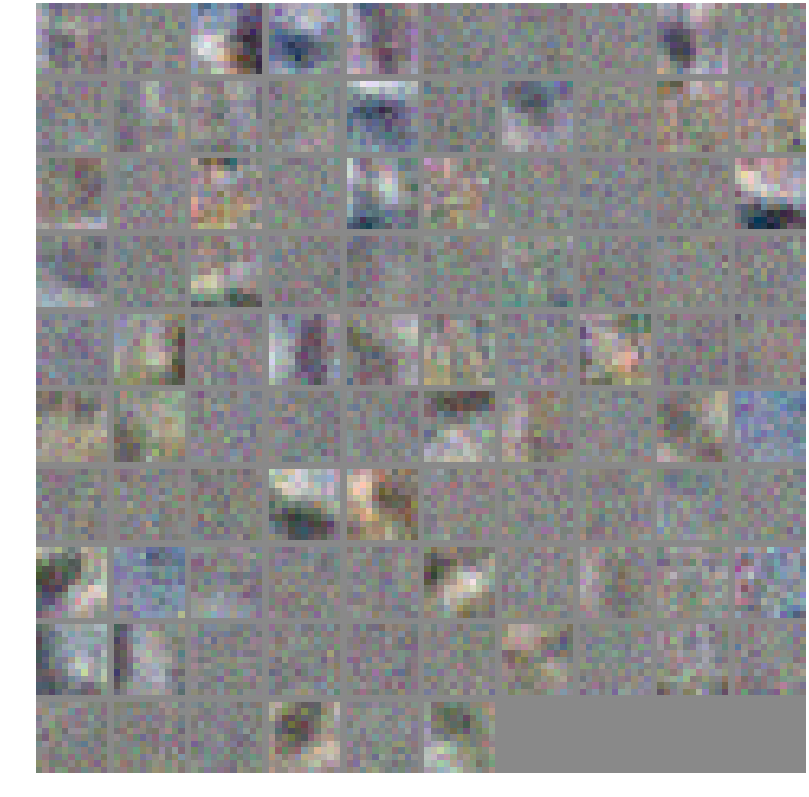
\includegraphics[width=0.49\textwidth]{images/grp0_conv1_weights_color.png}
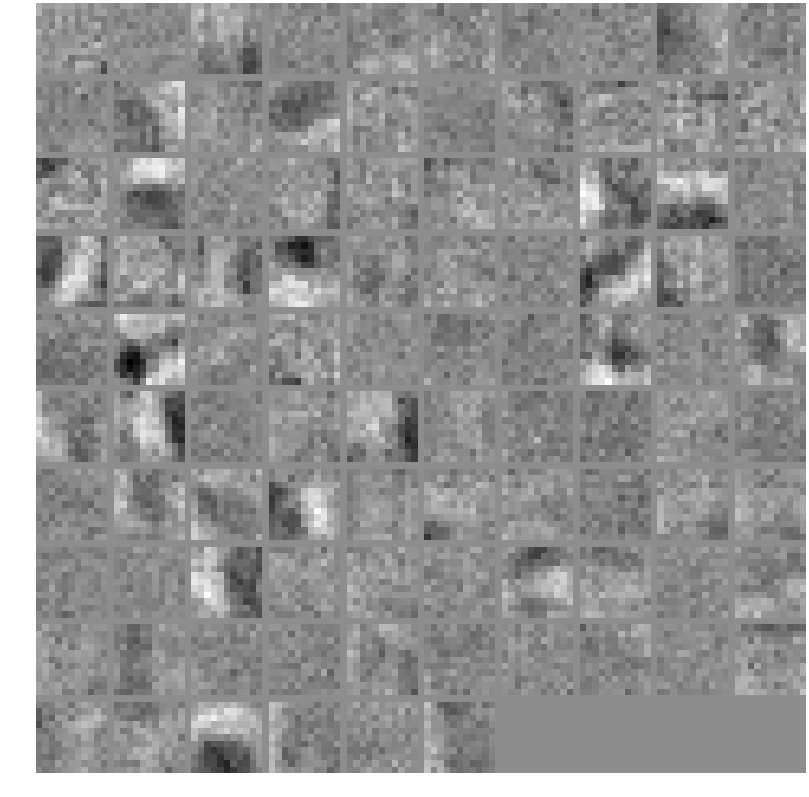
\includegraphics[width=0.49\textwidth]{images/grp0_conv1_weights_gray.png}
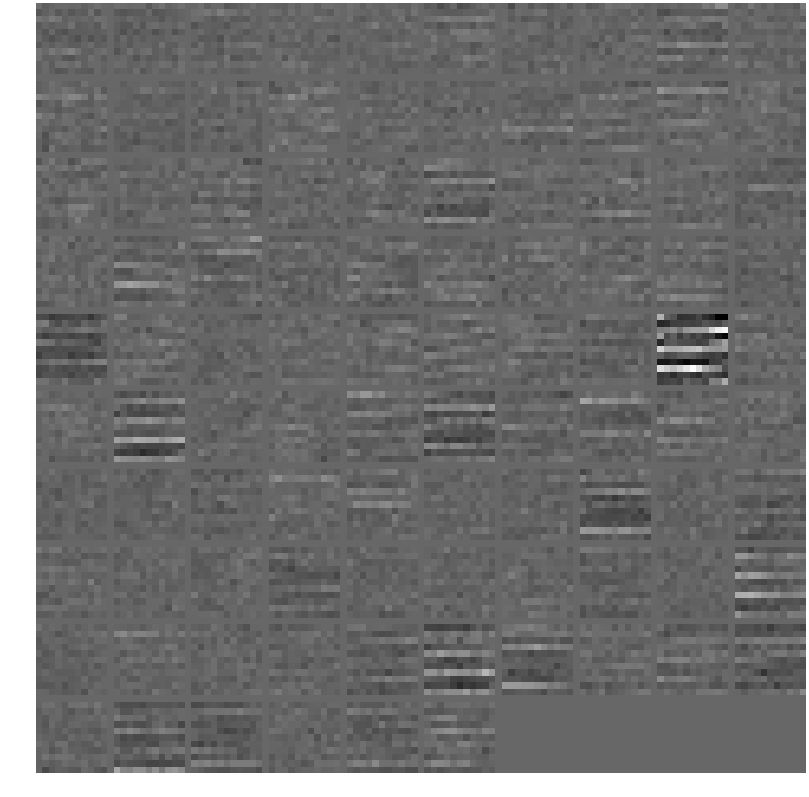
\includegraphics[width=0.49\textwidth]{images/grp0_conv1_weights_lid.png}
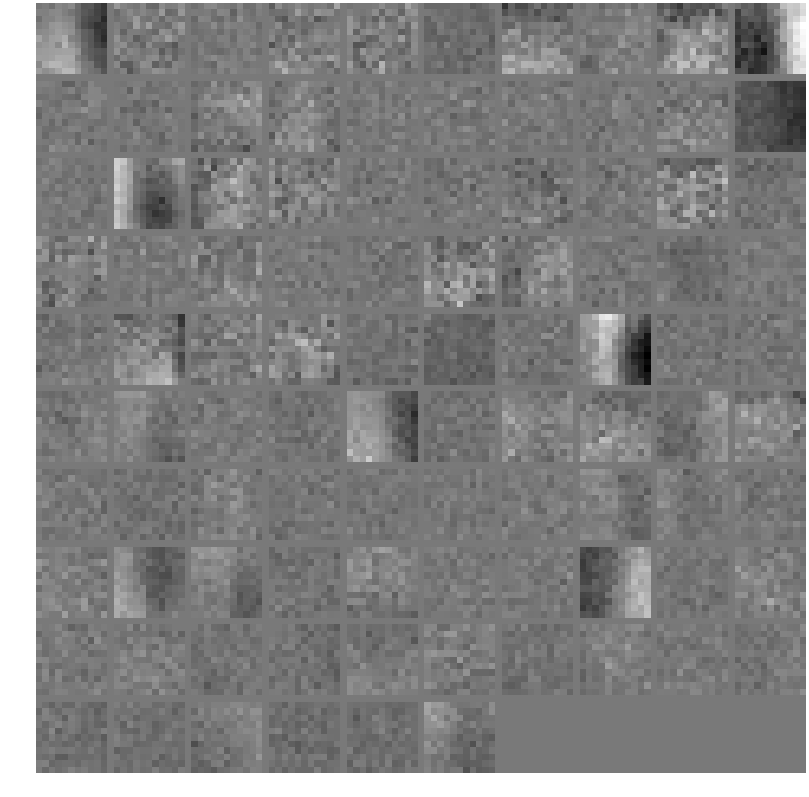
\includegraphics[width=0.49\textwidth]{images/grp0_conv1_weights_lid_depth.png}
\caption{Weights of the first convolutional layer of different feature maps, from top-left to bottom-right: color, grayscale, lidar and interpolated lidar}
\label{fig:filters}
\end{figure}

With the several millions of parameters contained in a neural network, this is not a particularly easy task. However several methods have been developed to visualize neural networks. The simplest and remarkably effective way to investigate the strength of the learning is to look at the first-order convolutional layers. The filters in those layers are applied directly on the image and they therefore contain first-level patterns the network learns. The first-order filters that are learned from some of the main individual feature maps are shown in Figure \ref{fig:filters}. Note first that all of the maps, except the images from the color camera, do only have one layer and are therefore shown in grayscale. 

It is immediately clear that several general filters are learned, but the filters are not all strong and some are relatively noisy. Focusing on the filters from the color images, it is clear that those color images do not really add significant information compared to the grayscale versions, as there are barely real color filters and instead mostly structural filters in several color variations. Only one blue filter is present, which appears to trigger on the sky. On the lidar filters the strength of the interpolation preprocessing is apparent, the non-interpolated version has only some noisy ribbed filters, showing the apparent complexity of handling the preprocessing with the network. In any case, for all networks more than half of the filters are considered 'dead' as they only contain a noise pattern. Thus only some edge and corner filters are learned, suggesting that a limited number of filters is apparently adequate for solving the task. This is especially visible with the interpolated filters, that contain mostly low-level filters with only vertical edges, indicating that these are apparently sufficient. Thus while the networks perform well on this data source, the task may actually be too easy to learn a rich representation from this feature map.
%Approximately half of the filters can however be considered 'dead' as they contain only a noise pattern, from which it appears only a limited number of filters is apparently adequate for solving the task.

\begin{figure}[t]
\centering
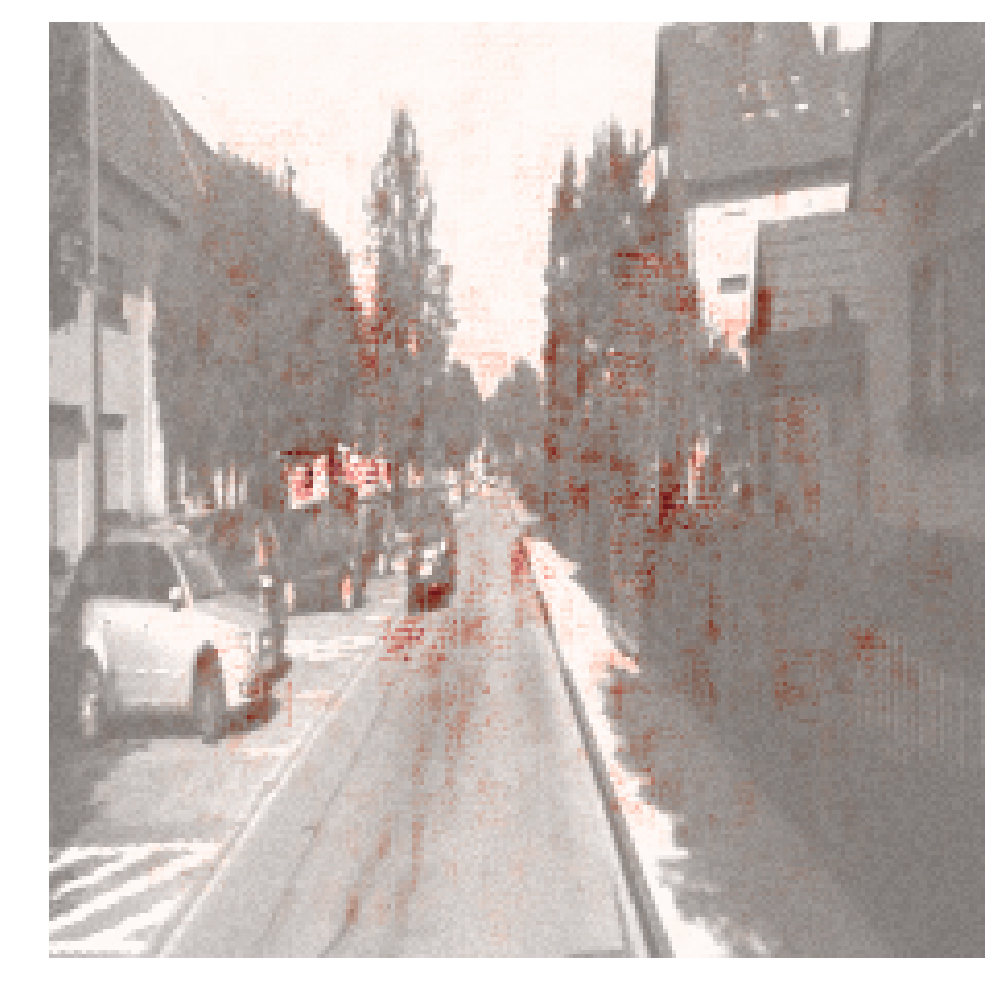
\includegraphics[width=0.49\textwidth]{images/saliency_1-0.png}
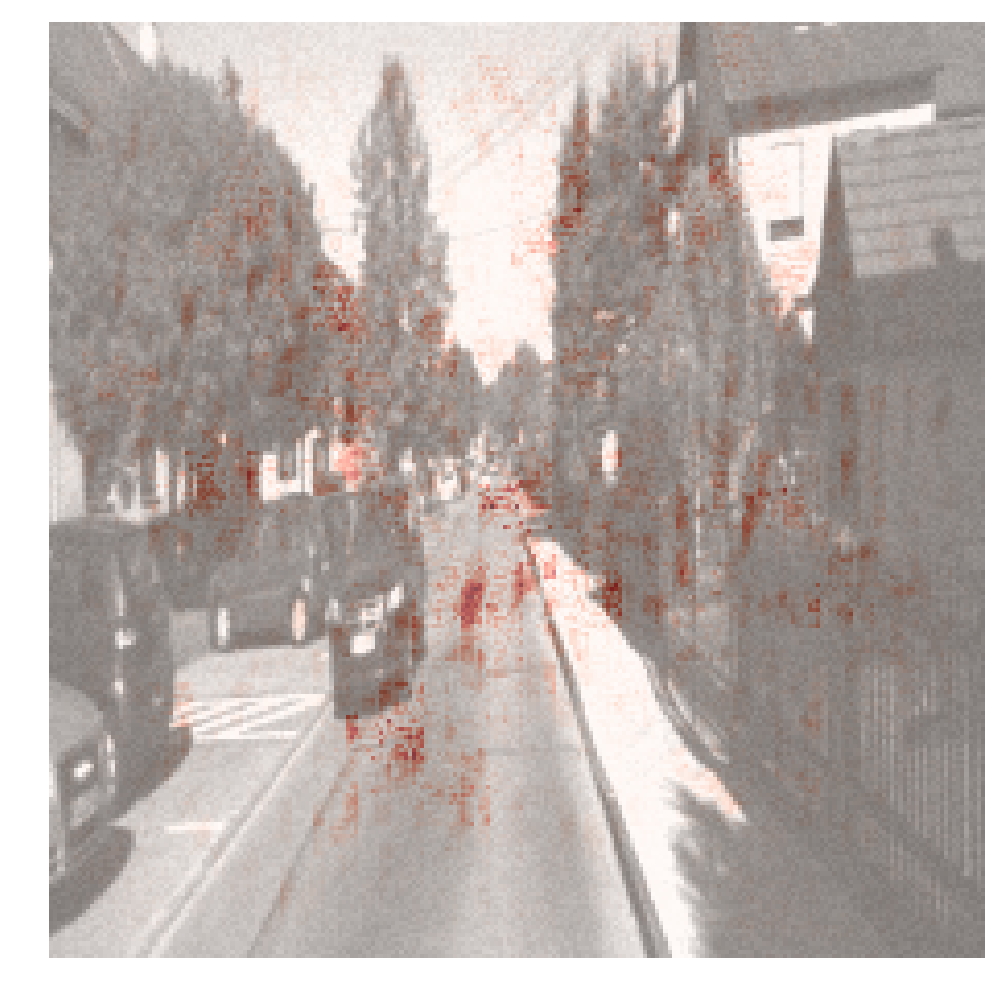
\includegraphics[width=0.49\textwidth]{images/saliency_1-1.png}
\caption{Saliency maps on the grayscale feature maps of two frames in the sequence shown in Figure \ref{fig:frames}, the darker the red colour the stronger the pixel influences the output permutation}
\label{fig:saliency}
\end{figure}

To investigate in more detail where the network focuses on, an alternative visualizing technique is investigated: saliency maps. Figure \ref{fig:saliency} shows saliency maps on the grayscale version in two frames. The saliency map should give an indication of the most important part of the image, but it is evident that the saliency map does not show particular attention to a certain kind of high-level feature, for example cars. There is also not a very apparent overlap between the same objects tracked through multiple frames in the sequence. The most important part of the image often appear at the center of every single frame, but this could have been anticipated as those parts should appear in multiple frames making it possible to compare them. It could however also suggest that a zoom-in might be used directly to compare the frames. This could indicate that the sequences have too little dynamic movement, as it appears that the network is partly ignoring the moving car, and instead finds the parts which remain static in both images. It should however be noted that the saliency maps do not appear to have been applied in this context before and there exists therefore no relevant literature to verify the applicability of this approach for this task.

Directly correlating corresponding parts in the image would be an foreseen approach, but it is is not expected to be so efficient, given the complex movement around the streets, with cars passing in the other direction, traffic crossing the street and the car turning in turns. While the saliency map seems to indicate that the indirect correlation approach comparing the relatively simple patterns learned from the backbone network between the different images might be a strong approach, this does not explain the high accuracy in turns reported in the previous section, because direct correlation of a zoom-in version does not work in that respect. 

%but this picture seems to indicate that the indirect correlation approach comparing the relatively simple patterns learned from the backbone network between the different images might still be a strong approach. It is however hard to conclude this confidently, as the saliency maps do not necessarily give the complete picture. Moreover, this technique has not been applied in this context before and there exists therefore no relevant literature to verify the applicability of this approach in this context.

\begin{figure}[t!]
\centering
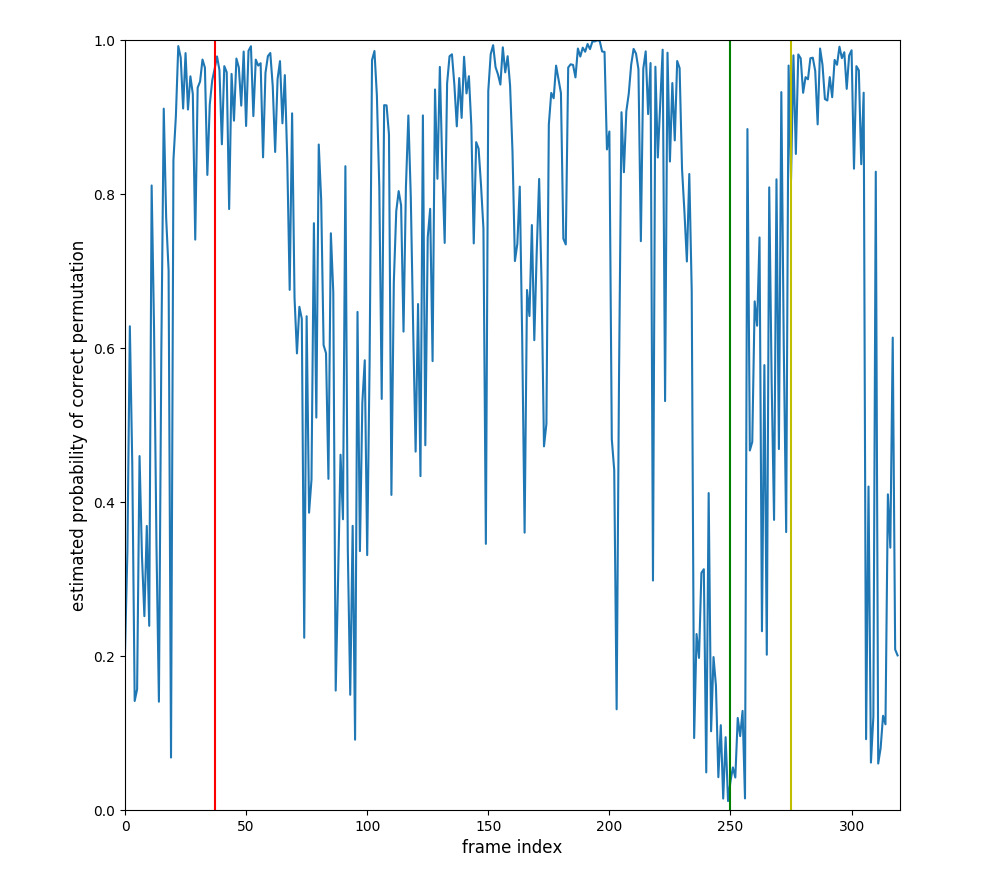
\includegraphics[width=\textwidth]{images/percentages_small.png}
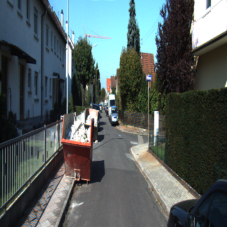
\includegraphics[width=0.32\textwidth]{images/000037.png}
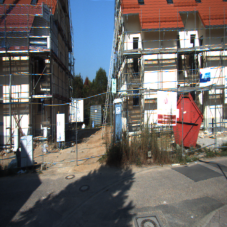
\includegraphics[width=0.32\textwidth]{images/000250.png}
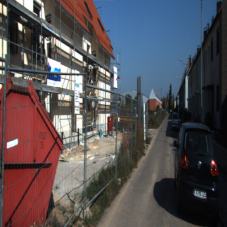
\includegraphics[width=0.32\textwidth]{images/000275.png}
\caption{Estimated probability of the sorted order of 4 frames of interpolated lidar depth given as input from the first 320 frames of sequence 15 with the index indicating the number of the first frame (top). On the bottom three images are shown with the left corresponding to the red line, the second to the green line and the third one to the yellow line}
\label{fig:percentages}
\end{figure}

To check the performance in different conditions a new test set has been created, starting at every frame from a particular sequence in sorted order. The probability is measured that the network correctly confirms that the frames are sorted (note that giving the items in sorted order might appear like an easier task, but the network has not been trained with any preference for sorted sequences). The result on the first 320 frames of sequence 15 are shown in Figure \ref{fig:percentages}. From the graph it clearly follows that there are  sections in the sequence where the network performs better (reaching close to 100\% accuracy) and worse, but there are also sections where the probability has sudden peaks. Color images of three frames in the sequence are also shown (please note that the data itself is trained on the interpolated lidar depth). It is not directly trivial to see why the specified sections are easy or hard. In the first image showing a region with high accuracy the network seems to work well around the red storage box, but it would be highly unlikely the network focuses on storage boxes. At the end of the road the accuracy is low, possibly due to the lack of a proper road (with a house under construction instead). Between the second and third image the car is turning, from which it is clear that during the turn results are bumpy, but still better than before the turn. Afterwards strong results are achieved for a certain timespan, but it is again not obvious what makes this part easier. 

Several techniques to visualize the behavior of the neural network were attempted, but it remains difficult to get a deeper understanding of the performance of the network. Therefore it is unfortunately hard to conclude where the relatively strong performance on the task exactly comes from. The learned filters show some generic patterns, but seem in general of limited strength and that makes it questionable if the network in the current state could be adopted for fine-tuning.


%A similar approach to find the important regions on the image is to find the location of the maximal activated neurons in the higher layers, for example in the fifth convolutional layer. For comparison with the previous approach the 5 maximal regions are shown for one of the frames investigated with the saliency map is shown in Figure \needfig. It is again hard to point which features the network is exactly focusing on, but there seems again a general tendency on several general static objects, for example trees around and the contour in the road. It remains however difficult to generalize a particular feature over multiple frames.

%% ----------------------------------------------------------------------------
% BIWI SA/MA thesis template
%
% Created 09/29/2006 by Andreas Ess
% Extended 13/02/2009 by Jan Lesniak - jlesniak@vision.ee.ethz.ch
%% ----------------------------------------------------------------------------

\chapter{Conclusions and Future Work}
In this work the applicability of self-supervised learning using an ordening task on camera and lidar data was analyzed with the autonomous driving dataset Kitti\cite{geiger2012}. The primary goal was twofold: (1) investigating the performance of a self-supervised task on an autonomous driving dataset and (2) researching the strength of additional input features in the form of lidar data in various representations and examining if those could enhance performance when combined with camera data.

It has been shown that the network are definitely capable of learning to order frames, the binary ordering task has even been shown to be on the easy side for a convolutional neural network to learn. Using the more difficult 24-order permutation task studied [??] top-1 accuracies were achieved, signalling strong and robust performance. The strong performance on the self-supervised task does unfortuantely however not appear to be directly scalable to different problems in its current state. It was found that the quality of the network filters remain on a relatively basic scale. Also more detailed investigations seem to indicate that the network does not learn details about particular objects and instead remain reliant on general correlation between images. To verify this behavior and to work on alternative approaches to make it harder to learn low-level features is an interesting direction for future work. Especially sampling different parts of the frame might be an worthwhile approach to investigate, although that would also imply getting rid of certain features in the field-of-view of the cameras making it impossible to use the frame consistency that is specifically apparent in driving datasets.  

From the point of view of using lidar to enhance the learning, it is directly clear that it improves the learning. [...]

The most important step for future work would be to test the investigated backbones on various alternative tasks like classification and object detection, to gain from the structure learnt by the self-supervised task, without direct supervision. Due to time constraints this step could unfortunately not yet been implemented as part of this thesis.


%% ----------------------------------------------------------------------------
% Bibliography is stored in references.bib file, and can often be found
% online on webpages like dblp.uni-trier.de
%
% To include it in your thesis, run
%  pdflatex main
%  bibtex main
%  pdflatex main
%  pdflatex main
%
% This ensures all references are done correctly.
%% ----------------------------------------------------------------------------

%\bibliographystyle{plain}
%\bibliography{references}
\addcontentsline{toc}{chapter}{\numberline{}{\noexpand Bibliography}}%}
\printbibliography


%% ----------------------------------------------------------------------------
% If Appendix is needed
%% ----------------------------------------------------------------------------
\appendix
%% ----------------------------------------------------------------------------
% BIWI SA/MA thesis template
%
% Created 09/29/2006 by Andreas Ess
% Extended 13/02/2009 by Jan Lesniak - jlesniak@vision.ee.ethz.ch
%% ----------------------------------------------------------------------------
\chapter{Implementation details}
\label{app:implementation_details}

The software produced for this thesis can be found at \needref. To use the software, reproduce the results in this thesis or to run new experiments the following steps should be followed:
\begin{enumerate}
\item The input data should be preprocessed to the correct format, to prevent expensive preprocessing while the network is learning. For this the scripts in the \textit{prepare/data} directory are useful. They read in the images from a central location and scale them down to 227x227 size, including possible conversion to grayscale before storing them on the disk.
\item Then the required training and test set can be generated. Herefore scripts are provided in the the \textit{prepare/input} directory for different varieties of the experiments.
\item In the next step the actual different type of experiments can be generated, for this purpose an \textit{generate/gen\_experiment.py} script is provided that initializes a directory with a solver.txt and net.txt protobuf files necessary for running Caffe. All the experiments are found in the \textit{experiments} folder, where relevant paths should be updated to reflect the appropriate local file system.
\item Eventually the training can be run by invoking \textit{train.py} with the first argument to the solver.txt of the generated experiment. 
\item Finally when training is finished, accuracy can be calculated and some of the visualizations can be produced by running \textit{test.py} with the first argument pointing to the net.prototxt and the second argument a .caffemodel file produced during training that contain the state of the network.
\end{enumerate}
All the software is made available under the MIT license. Note that the software is considered research in progress and has limited documentation. Several small changes might be required to allow running the software stack on your own computer, however everything to reproduce the overall results in this work should be present.


\end{document}

